\section{ARQUITETURA DA INFRAESTRUTURA}

\subsection{Topologia Física e Lógica}

A infraestrutura é constituída por 22 dispositivos interconectados através de 23 enlaces:
\begin{itemize}[leftmargin=2em]
  \item \textbf{Núcleo WAN (R0 a R3):} 4 roteadores modelo \textit{Router-PT-Empty} equipados com módulos seriais inteligentes (\texttt{PT-ROUTER-NM-1SS}), formando uma topologia de malha completa (\textit{full-mesh}) com 6 enlaces seriais ponto a ponto.
  \item \textbf{Roteadores de Borda (R4 a R7):} 4 roteadores de borda responsáveis pelo atendimento das LANs departamentais, cada um conectado por enlace serial a um roteador de núcleo específico e por interface GigabitEthernet ao respectivo switch de acesso.
  \item \textbf{Comutadores de Acesso (Switch0 a Switch3):} 4 switches modelo \textit{Switch-PT-Empty} com portas GigabitEthernet interligando as estações de trabalho e os roteadores de borda.
  \item \textbf{Estações Finais (PC0 a PC8):} 9 computadores com conectividade FastEthernet recebendo endereçamento dinâmico via pools DHCP configurados nos roteadores de borda.
\end{itemize}

\begin{figure}[H]
    \centering
    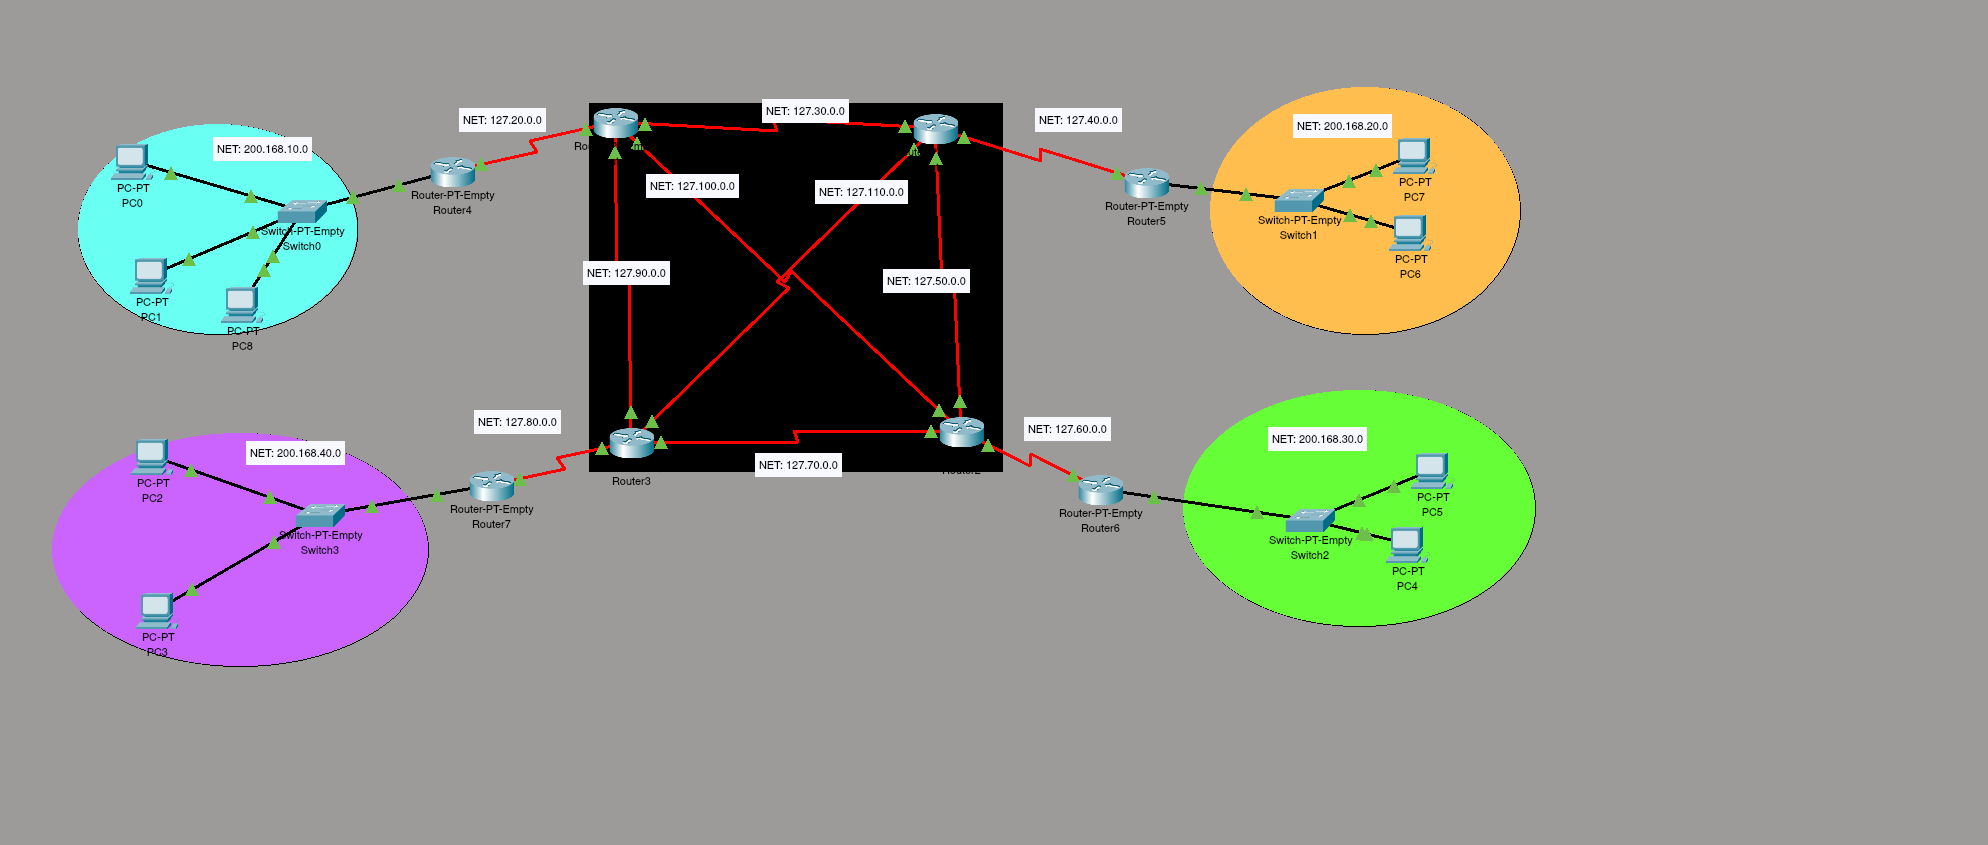
\includegraphics[width=0.85\linewidth]{pics/cenario_real.png}
    \caption{Topologia física do Cenário 02 no Cisco Packet Tracer.}
    \label{fig:topologia_real}
\end{figure}

\subsection{Interfaces e Endereçamento de Roteadores}

A Tabela~\ref{tab:ifaces} detalha a distribuição das 24 interfaces de roteamento ativas, seus endereços IPv4, máscaras e larguras de banda atribuídas aos enlaces.

\begin{table}[H]
\centering
\small
\begin{tabular}{llllll}
\toprule
Roteador & Interface & IP & Prefixo & Banda & Clock/Tipo\\
\midrule
R0 & Serial6/0 & 172.30.0.1 & /16 & 1544 kb/s & DCE\\
R0 & Serial7/0 & 172.20.0.2 & /16 & 1544 kb/s & DCE\\
R0 & Serial8/0 & 172.100.0.1 & /16 & 1544 kb/s & DCE\\
R0 & Serial9/0 & 172.90.0.2 & /16 & 1544 kb/s & DTE\\
\midrule
R1 & Serial6/0 & 172.30.0.2 & /16 & 1544 kb/s & DTE\\
R1 & Serial7/0 & 172.50.0.1 & /16 & 1544 kb/s & DCE\\
R1 & Serial8/0 & 172.110.0.1 & /16 & 1544 kb/s & DTE\\
R1 & Serial9/0 & 172.40.0.2 & /16 & 1544 kb/s & DCE\\
\midrule
R2 & Serial6/0 & 172.60.0.2 & /16 & 1544 kb/s & DCE\\
R2 & Serial7/0 & 172.50.0.2 & /16 & 1544 kb/s & DTE\\
R2 & Serial8/0 & 172.70.0.1 & /16 & 1544 kb/s & DCE\\
R2 & Serial9/0 & 172.100.0.2 & /16 & 1544 kb/s & DTE\\
\midrule
R3 & Serial6/0 & 172.80.0.2 & /16 & 1544 kb/s & DTE\\
R3 & Serial7/0 & 172.110.0.2 & /16 & 1544 kb/s & DCE\\
R3 & Serial8/0 & 172.70.0.2 & /16 & 1544 kb/s & DTE\\
R3 & Serial9/0 & 172.90.0.1 & /16 & 1544 kb/s & DCE\\
\midrule
R4 & Serial0/0 & 172.20.0.1 & /16 & 1544 kb/s & DTE\\
R4 & GigabitEthernet9/0 & 200.168.10.254 & /24 & 1 Gb/s & --\\
\midrule
R5 & Serial0/0 & 172.40.0.1 & /16 & 1544 kb/s & DTE\\
R5 & GigabitEthernet9/0 & 200.168.20.254 & /24 & 1 Gb/s & --\\
\midrule
R6 & Serial0/0 & 172.60.0.1 & /16 & 1544 kb/s & DTE\\
R6 & GigabitEthernet9/0 & 200.168.30.254 & /24 & 1 Gb/s & --\\
\midrule
R7 & Serial0/0 & 172.80.0.1 & /16 & 1544 kb/s & DCE\\
R7 & GigabitEthernet9/0 & 200.168.40.254 & /24 & 1 Gb/s & --\\
\bottomrule
\end{tabular}

\caption{Interfaces dos roteadores e enlaces de interconexão.}
\label{tab:ifaces}
\end{table}

\subsection{Portas de Switch e Estações de Trabalho}

A Tabela~\ref{tab:switchports} resume a ocupação de portas nos switches de acesso, e a Tabela~\ref{tab:pcs} apresenta as estações de trabalho conectadas a cada equipamento.

\begin{table}[H]
\centering
\small
\begin{tabular}{llll}
\toprule
Switch & Porta & Banda & Conectado a\\
\midrule
Switch0 & Gi0/1 & 1 Gb/s & R4 GigabitEthernet9/0\\
Switch0 & Gi7/1 & 100 Mb/s & PC8 FastEthernet0\\
Switch0 & Gi8/1 & 100 Mb/s & PC1 FastEthernet0\\
Switch0 & Gi9/1 & 100 Mb/s & PC0 FastEthernet0\\
\midrule
Switch1 & Gi0/1 & 100 Mb/s & PC7 FastEthernet0\\
Switch1 & Gi7/1 & 100 Mb/s & PC6 FastEthernet0\\
Switch1 & Gi8/1 & 1 Gb/s & livre\\
Switch1 & Gi9/1 & 1 Gb/s & R5 GigabitEthernet9/0\\
\midrule
Switch2 & Gi0/1 & 100 Mb/s & PC5 FastEthernet0\\
Switch2 & Gi7/1 & 100 Mb/s & PC4 FastEthernet0\\
Switch2 & Gi8/1 & 1 Gb/s & livre\\
Switch2 & Gi9/1 & 1 Gb/s & R6 GigabitEthernet9/0\\
\midrule
Switch3 & Gi0/1 & 100 Mb/s & livre\\
Switch3 & Gi7/1 & 100 Mb/s & PC3 FastEthernet0\\
Switch3 & Gi8/1 & 100 Mb/s & PC2 FastEthernet0\\
Switch3 & Gi9/1 & 1 Gb/s & R7 GigabitEthernet9/0\\
\bottomrule
\end{tabular}

\caption{Mapeamento de portas dos comutadores.}
\label{tab:switchports}
\end{table}

\begin{table}[H]
\centering
\small
\begin{tabular}{ll}
\toprule
PC & Conectado ao Switch\\
\midrule
PC0 & Switch0 Gi9/1\\
PC1 & Switch0 Gi8/1\\
PC2 & Switch3 Gi8/1\\
PC3 & Switch3 Gi7/1\\
PC4 & Switch2 Gi7/1\\
PC5 & Switch2 Gi0/1\\
PC6 & Switch1 Gi7/1\\
PC7 & Switch1 Gi0/1\\
PC8 & Switch0 Gi7/1\\
\bottomrule
\end{tabular}

\caption{Estações de trabalho conectadas.}
\label{tab:pcs}
\end{table}

\section{ROTEAMENTO DINÂMICO E TABELA RIB}

O roteamento da infraestrutura baseia-se exclusivamente no protocolo OSPF processo 1 operando em área única (\textit{Area 0}). O custo OSPF dos enlaces seriais é determinado pela relação $\lfloor 10^8 / bw_{bps} \rfloor$, resultando no custo métrico padrão de 64 para links seriais T1 (1544 kb/s), e custo 1 para interfaces locais GigabitEthernet. As interfaces LAN dos roteadores de borda são configuradas como \texttt{passive-interface} para conter o tráfego de controle desnecessário nas redes de acesso.

\subsection{Base de Informações de Roteamento (RIB)}

A seguir são apresentadas as entradas calculadas da RIB esperada para os roteadores da topologia:

\subsection*{R0 (Router0)}
\begin{tabular}{@{}llllp{3.6cm}@{}}\toprule Destino & Cód. & Interface de saída & Métrica & Próximo salto\\\midrule
172.20.0.0/16 & C & Serial7/0 & -- & --\\
172.30.0.0/16 & C & Serial6/0 & -- & --\\
172.40.0.0/16 & O & Serial6/0 & 128 & 172.30.0.2\\
172.50.0.0/16 & O & Serial6/0, Serial8/0 & 128 & 172.30.0.2, 172.100.0.2\\
172.60.0.0/16 & O & Serial8/0 & 128 & 172.100.0.2\\
172.70.0.0/16 & O & Serial8/0, Serial9/0 & 128 & 172.100.0.2, 172.90.0.1\\
172.80.0.0/16 & O & Serial9/0 & 128 & 172.90.0.1\\
172.90.0.0/16 & C & Serial9/0 & -- & --\\
172.100.0.0/16 & C & Serial8/0 & -- & --\\
172.110.0.0/16 & O & Serial6/0, Serial9/0 & 128 & 172.30.0.2, 172.90.0.1\\
200.168.10.0/24 & O & Serial7/0 & 65 & 172.20.0.1\\
200.168.20.0/24 & O & Serial6/0 & 129 & 172.30.0.2\\
200.168.30.0/24 & O & Serial8/0 & 129 & 172.100.0.2\\
200.168.40.0/24 & O & Serial9/0 & 129 & 172.90.0.1\\
\bottomrule\end{tabular}

\subsection*{R1 (Router1)}
\begin{tabular}{@{}llllp{3.6cm}@{}}\toprule Destino & Cód. & Interface de saída & Métrica & Próximo salto\\\midrule
172.20.0.0/16 & O & Serial6/0 & 128 & 172.30.0.1\\
172.30.0.0/16 & C & Serial6/0 & -- & --\\
172.40.0.0/16 & C & Serial9/0 & -- & --\\
172.50.0.0/16 & C & Serial7/0 & -- & --\\
172.60.0.0/16 & O & Serial7/0 & 128 & 172.50.0.2\\
172.70.0.0/16 & O & Serial7/0, Serial8/0 & 128 & 172.50.0.2, 172.110.0.2\\
172.80.0.0/16 & O & Serial8/0 & 128 & 172.110.0.2\\
172.90.0.0/16 & O & Serial6/0, Serial8/0 & 128 & 172.30.0.1, 172.110.0.2\\
172.100.0.0/16 & O & Serial6/0, Serial7/0 & 128 & 172.30.0.1, 172.50.0.2\\
172.110.0.0/16 & C & Serial8/0 & -- & --\\
200.168.10.0/24 & O & Serial6/0 & 129 & 172.30.0.1\\
200.168.20.0/24 & O & Serial9/0 & 65 & 172.40.0.1\\
200.168.30.0/24 & O & Serial7/0 & 129 & 172.50.0.2\\
200.168.40.0/24 & O & Serial8/0 & 129 & 172.110.0.2\\
\bottomrule\end{tabular}

\subsection*{R2 (Router2)}
\begin{tabular}{@{}llllp{3.6cm}@{}}\toprule Destino & Cód. & Interface de saída & Métrica & Próximo salto\\\midrule
172.20.0.0/16 & O & Serial9/0 & 128 & 172.100.0.1\\
172.30.0.0/16 & O & Serial9/0, Serial7/0 & 128 & 172.100.0.1, 172.50.0.1\\
172.40.0.0/16 & O & Serial7/0 & 128 & 172.50.0.1\\
172.50.0.0/16 & C & Serial7/0 & -- & --\\
172.60.0.0/16 & C & Serial6/0 & -- & --\\
172.70.0.0/16 & C & Serial8/0 & -- & --\\
172.80.0.0/16 & O & Serial8/0 & 128 & 172.70.0.2\\
172.90.0.0/16 & O & Serial9/0, Serial8/0 & 128 & 172.100.0.1, 172.70.0.2\\
172.100.0.0/16 & C & Serial9/0 & -- & --\\
172.110.0.0/16 & O & Serial7/0, Serial8/0 & 128 & 172.50.0.1, 172.70.0.2\\
200.168.10.0/24 & O & Serial9/0 & 129 & 172.100.0.1\\
200.168.20.0/24 & O & Serial7/0 & 129 & 172.50.0.1\\
200.168.30.0/24 & O & Serial6/0 & 65 & 172.60.0.1\\
200.168.40.0/24 & O & Serial8/0 & 129 & 172.70.0.2\\
\bottomrule\end{tabular}

\subsection*{R3 (Router3)}
\begin{tabular}{@{}llllp{3.6cm}@{}}\toprule Destino & Cód. & Interface de saída & Métrica & Próximo salto\\\midrule
172.20.0.0/16 & O & Serial9/0 & 128 & 172.90.0.2\\
172.30.0.0/16 & O & Serial9/0, Serial7/0 & 128 & 172.90.0.2, 172.110.0.1\\
172.40.0.0/16 & O & Serial7/0 & 128 & 172.110.0.1\\
172.50.0.0/16 & O & Serial7/0, Serial8/0 & 128 & 172.110.0.1, 172.70.0.1\\
172.60.0.0/16 & O & Serial8/0 & 128 & 172.70.0.1\\
172.70.0.0/16 & C & Serial8/0 & -- & --\\
172.80.0.0/16 & C & Serial6/0 & -- & --\\
172.90.0.0/16 & C & Serial9/0 & -- & --\\
172.100.0.0/16 & O & Serial9/0, Serial8/0 & 128 & 172.90.0.2, 172.70.0.1\\
172.110.0.0/16 & C & Serial7/0 & -- & --\\
200.168.10.0/24 & O & Serial9/0 & 129 & 172.90.0.2\\
200.168.20.0/24 & O & Serial7/0 & 129 & 172.110.0.1\\
200.168.30.0/24 & O & Serial8/0 & 129 & 172.70.0.1\\
200.168.40.0/24 & O & Serial6/0 & 65 & 172.80.0.1\\
\bottomrule\end{tabular}

\subsection*{R4 (Router4)}
\begin{tabular}{@{}llllp{3.6cm}@{}}\toprule Destino & Cód. & Interface de saída & Métrica & Próximo salto\\\midrule
172.20.0.0/16 & C & Serial0/0 & -- & --\\
172.30.0.0/16 & O & Serial0/0 & 128 & 172.20.0.2\\
172.40.0.0/16 & O & Serial0/0 & 192 & 172.20.0.2\\
172.50.0.0/16 & O & Serial0/0 & 192 & 172.20.0.2\\
172.60.0.0/16 & O & Serial0/0 & 192 & 172.20.0.2\\
172.70.0.0/16 & O & Serial0/0 & 192 & 172.20.0.2\\
172.80.0.0/16 & O & Serial0/0 & 192 & 172.20.0.2\\
172.90.0.0/16 & O & Serial0/0 & 128 & 172.20.0.2\\
172.100.0.0/16 & O & Serial0/0 & 128 & 172.20.0.2\\
172.110.0.0/16 & O & Serial0/0 & 192 & 172.20.0.2\\
200.168.10.0/24 & C & GigabitEthernet9/0 & -- & --\\
200.168.20.0/24 & O & Serial0/0 & 193 & 172.20.0.2\\
200.168.30.0/24 & O & Serial0/0 & 193 & 172.20.0.2\\
200.168.40.0/24 & O & Serial0/0 & 193 & 172.20.0.2\\
\bottomrule\end{tabular}

\subsection*{R5 (Router5)}
\begin{tabular}{@{}llllp{3.6cm}@{}}\toprule Destino & Cód. & Interface de saída & Métrica & Próximo salto\\\midrule
172.20.0.0/16 & O & Serial0/0 & 192 & 172.40.0.2\\
172.30.0.0/16 & O & Serial0/0 & 128 & 172.40.0.2\\
172.40.0.0/16 & C & Serial0/0 & -- & --\\
172.50.0.0/16 & O & Serial0/0 & 128 & 172.40.0.2\\
172.60.0.0/16 & O & Serial0/0 & 192 & 172.40.0.2\\
172.70.0.0/16 & O & Serial0/0 & 192 & 172.40.0.2\\
172.80.0.0/16 & O & Serial0/0 & 192 & 172.40.0.2\\
172.90.0.0/16 & O & Serial0/0 & 192 & 172.40.0.2\\
172.100.0.0/16 & O & Serial0/0 & 192 & 172.40.0.2\\
172.110.0.0/16 & O & Serial0/0 & 128 & 172.40.0.2\\
200.168.10.0/24 & O & Serial0/0 & 193 & 172.40.0.2\\
200.168.20.0/24 & C & GigabitEthernet9/0 & -- & --\\
200.168.30.0/24 & O & Serial0/0 & 193 & 172.40.0.2\\
200.168.40.0/24 & O & Serial0/0 & 193 & 172.40.0.2\\
\bottomrule\end{tabular}

\subsection*{R6 (Router6)}
\begin{tabular}{@{}llllp{3.6cm}@{}}\toprule Destino & Cód. & Interface de saída & Métrica & Próximo salto\\\midrule
172.20.0.0/16 & O & Serial0/0 & 192 & 172.60.0.2\\
172.30.0.0/16 & O & Serial0/0 & 192 & 172.60.0.2\\
172.40.0.0/16 & O & Serial0/0 & 192 & 172.60.0.2\\
172.50.0.0/16 & O & Serial0/0 & 128 & 172.60.0.2\\
172.60.0.0/16 & C & Serial0/0 & -- & --\\
172.70.0.0/16 & O & Serial0/0 & 128 & 172.60.0.2\\
172.80.0.0/16 & O & Serial0/0 & 192 & 172.60.0.2\\
172.90.0.0/16 & O & Serial0/0 & 192 & 172.60.0.2\\
172.100.0.0/16 & O & Serial0/0 & 128 & 172.60.0.2\\
172.110.0.0/16 & O & Serial0/0 & 192 & 172.60.0.2\\
200.168.10.0/24 & O & Serial0/0 & 193 & 172.60.0.2\\
200.168.20.0/24 & O & Serial0/0 & 193 & 172.60.0.2\\
200.168.30.0/24 & C & GigabitEthernet9/0 & -- & --\\
200.168.40.0/24 & O & Serial0/0 & 193 & 172.60.0.2\\
\bottomrule\end{tabular}

\subsection*{R7 (Router7)}
\begin{tabular}{@{}llllp{3.6cm}@{}}\toprule Destino & Cód. & Interface de saída & Métrica & Próximo salto\\\midrule
172.20.0.0/16 & O & Serial0/0 & 192 & 172.80.0.2\\
172.30.0.0/16 & O & Serial0/0 & 192 & 172.80.0.2\\
172.40.0.0/16 & O & Serial0/0 & 192 & 172.80.0.2\\
172.50.0.0/16 & O & Serial0/0 & 192 & 172.80.0.2\\
172.60.0.0/16 & O & Serial0/0 & 192 & 172.80.0.2\\
172.70.0.0/16 & O & Serial0/0 & 128 & 172.80.0.2\\
172.80.0.0/16 & C & Serial0/0 & -- & --\\
172.90.0.0/16 & O & Serial0/0 & 128 & 172.80.0.2\\
172.100.0.0/16 & O & Serial0/0 & 192 & 172.80.0.2\\
172.110.0.0/16 & O & Serial0/0 & 128 & 172.80.0.2\\
200.168.10.0/24 & O & Serial0/0 & 193 & 172.80.0.2\\
200.168.20.0/24 & O & Serial0/0 & 193 & 172.80.0.2\\
200.168.30.0/24 & O & Serial0/0 & 193 & 172.80.0.2\\
200.168.40.0/24 & C & GigabitEthernet9/0 & -- & --\\
\bottomrule\end{tabular}


\subsection{Configurações dos Roteadores (Running-Configs)}

A listagem a seguir apresenta as configurações essenciais extraídas diretamente dos dispositivos no arquivo Packet Tracer, compreendendo os endereçamentos, escopos DHCP locais e parâmetros OSPF:

\subsection*{Router0}
\begin{lstlisting}
hostname R0
interface Serial6/0
 ip address 172.30.0.1 255.255.0.0
 clock rate 2000000
interface Serial7/0
 ip address 172.20.0.2 255.255.0.0
 clock rate 4000000
interface Serial8/0
 ip address 172.100.0.1 255.255.0.0
 clock rate 2000000
interface Serial9/0
 ip address 172.90.0.2 255.255.0.0
router ospf 1
 router-id 1.1.1.1
 network 172.0.0.0 0.255.255.255 area 0
\end{lstlisting}
\subsection*{Router1}
\begin{lstlisting}
hostname R1
interface Serial6/0
 ip address 172.30.0.2 255.255.0.0
interface Serial7/0
 ip address 172.50.0.1 255.255.0.0
 clock rate 2000000
interface Serial8/0
 ip address 172.110.0.1 255.255.0.0
interface Serial9/0
 ip address 172.40.0.2 255.255.0.0
 clock rate 2000000
router ospf 1
 router-id 2.2.2.2
 network 172.0.0.0 0.255.255.255 area 0
\end{lstlisting}
\subsection*{Router2}
\begin{lstlisting}
hostname R2
interface Serial6/0
 ip address 172.60.0.2 255.255.0.0
 clock rate 2000000
interface Serial7/0
 ip address 172.50.0.2 255.255.0.0
interface Serial8/0
 ip address 172.70.0.1 255.255.0.0
 clock rate 2000000
interface Serial9/0
 ip address 172.100.0.2 255.255.0.0
router ospf 1
 router-id 3.3.3.3
 network 172.0.0.0 0.255.255.255 area 0
\end{lstlisting}
\subsection*{Router3}
\begin{lstlisting}
hostname R3
interface Serial6/0
 ip address 172.80.0.2 255.255.0.0
interface Serial7/0
 ip address 172.110.0.2 255.255.0.0
 clock rate 2000000
interface Serial8/0
 ip address 172.70.0.2 255.255.0.0
interface Serial9/0
 ip address 172.90.0.1 255.255.0.0
 clock rate 2000000
router ospf 1
 router-id 4.4.4.4
 network 172.0.0.0 0.255.255.255 area 0
\end{lstlisting}
\subsection*{Router4}
\begin{lstlisting}
hostname R4
ip dhcp excluded-address 200.168.10.1
ip dhcp excluded-address 200.168.10.2
ip dhcp excluded-address 200.168.10.3
ip dhcp excluded-address 200.168.10.254
ip dhcp excluded-address 200.168.10.1 200.168.10.3
ip dhcp pool REDE_LOCAL_10
 network 200.168.10.0 255.255.255.0
 default-router 200.168.10.254
 dns-server 8.8.8.8
interface Serial0/0
 ip address 172.20.0.1 255.255.0.0
interface GigabitEthernet9/0
 ip address 200.168.10.254 255.255.255.0
router ospf 1
 router-id 5.5.5.5
 passive-interface GigabitEthernet9/0
 network 172.0.0.0 0.255.255.255 area 0
 network 200.168.10.0 0.0.0.255 area 0
\end{lstlisting}
\subsection*{Router5}
\begin{lstlisting}
hostname R5
ip dhcp excluded-address 200.168.20.254
ip dhcp pool REDE_LOCAL_20
 network 200.168.20.0 255.255.255.0
 default-router 200.168.20.254
 dns-server 8.8.8.8
interface Serial0/0
 ip address 172.40.0.1 255.255.0.0
interface GigabitEthernet9/0
 ip address 200.168.20.254 255.255.255.0
router ospf 1
 router-id 6.6.6.6
 passive-interface GigabitEthernet9/0
 network 172.0.0.0 0.255.255.255 area 0
 network 200.168.20.0 0.0.0.255 area 0
\end{lstlisting}
\subsection*{Router6}
\begin{lstlisting}
hostname R6
ip dhcp excluded-address 200.168.30.254
ip dhcp pool REDE_LOCAL_30
 network 200.168.30.0 255.255.255.0
 default-router 200.168.30.254
 dns-server 8.8.8.8
interface Serial0/0
 ip address 172.60.0.1 255.255.0.0
interface GigabitEthernet9/0
 ip address 200.168.30.254 255.255.255.0
router ospf 1
 router-id 7.7.7.7
 passive-interface GigabitEthernet9/0
 network 172.0.0.0 0.255.255.255 area 0
 network 200.168.30.0 0.0.0.255 area 0
\end{lstlisting}
\subsection*{Router7}
\begin{lstlisting}
hostname R7
ip dhcp excluded-address 200.168.40.254
ip dhcp pool REDE_LOCAL_40
 network 200.168.40.0 255.255.255.0
 default-router 200.168.40.254
 dns-server 8.8.8.8
interface Serial0/0
 ip address 172.80.0.1 255.255.0.0
 clock rate 2000000
interface GigabitEthernet9/0
 ip address 200.168.40.254 255.255.255.0
router ospf 1
 router-id 8.8.8.8
 passive-interface GigabitEthernet9/0
 network 172.0.0.0 0.255.255.255 area 0
 network 200.168.40.0 0.0.0.255 area 0
\end{lstlisting}
